% ECML-PKDD Research track version (LNCS, 16pp incl. refs)
\documentclass[runningheads]{llncs}

\usepackage[T1]{fontenc}
\usepackage{lmodern}
\usepackage{graphicx}
\usepackage{amsmath,amssymb}
\usepackage{booktabs}
\usepackage{multirow}
\usepackage{float}
\usepackage{url}
\usepackage{xurl}
\emergencystretch=2em

% Relax float placement so large tables/figures pack densely instead of
% stranding float-only pages (helps hit the 16pp ECML-PKDD limit).
\renewcommand{\topfraction}{0.92}
\renewcommand{\bottomfraction}{0.85}
\renewcommand{\textfraction}{0.08}
\renewcommand{\floatpagefraction}{0.80}
\setcounter{topnumber}{3}
\setcounter{bottomnumber}{2}
\setcounter{totalnumber}{5}

\begin{document}

\title{Jigsaw: Retrieval-Constrained Exact Subgraph Matching}
\titlerunning{Jigsaw}
\author{}
\authorrunning{Anonymous}
\institute{}
\maketitle

\begin{abstract}
Exact subgraph-isomorphism solvers such as Glasgow are sound and complete, but a resident whole-graph candidate domain can exceed serving memory or overwhelm a verifier under a fixed time budget. On full OGBN-MAG (1.9M nodes), direct CP-based Glasgow solves \textbf{0 of 15} sampled queries; the same configuration does not finish on OGBN-Arxiv (169K, 0/15) yet solves Cora (19.8K, 15/15 in ${\approx}2.7$\,s). We introduce \textbf{Jigsaw}, a retrieval-constrained verifier: a GNN trained with \textbf{FullCov}, a coverage objective requiring every touched partition, retrieves hierarchical partitions; we stitch one-hop overlap, prune by typed signatures and exact labels, then invoke Glasgow. Jigsaw retains a retriever-agnostic interface because the strongest bounded ranker depends on \emph{label selectivity}: a classical label index dominates under near-unique labels ($96.7\%>$ learned $88.6\%$), while learned retrieval becomes the better localizer as labels coarsen. Across Cora, Arxiv, and MAG, Jigsaw makes most MAG queries exactly solvable ($88.6\%$ learned, $98.4\%$ exhaustive), remains exact inside the retrieved candidate, rejects audited negatives at $99.3$--$100.0\%$, and streams MAG at $2.4$\,GB rather than $10.2$\,GB for whole-graph residence.
\keywords{Subgraph isomorphism \and Graph neural networks \and Exact verification \and Neural retrieval}
\end{abstract}

\section{Introduction}

Subgraph isomorphism is used in motif discovery, scientific graph analysis, fraud search, and security auditing. Exact solvers are sound and complete but pay for large candidate domains; learned retrieval scales better but does not certify matches. Jigsaw composes the two: learned narrowing followed by exact verification.

Jigsaw partitions a large graph, embeds queries and partitions into a shared space, retrieves candidate partitions, stitches overlap neighborhoods, prunes by typed signatures and exact labels, and calls Glasgow. If retrieval covers the planted match, the verifier certifies the result inside the candidate; if retrieval misses a required region, local soundness remains but global completeness is lost. FullCov makes this coverage condition explicit.

We evaluate Cora, OGBN-Arxiv, and MAG with two seeds, three sizes, six positive and two negative families, and six retrieval policies. Cora/Arxiv reach $100\%$ only at the exhaustive all-partition budget; at the matched half-partition budget Jigsaw reaches $94.2/92.8/88.6\%$ on Cora/Arxiv/MAG.

\paragraph{Contributions.}
\begin{itemize}
    \item We scale exact subgraph matching to MAG via retrieval-constrained verification: direct Glasgow solves 0/15 MAG queries, while Jigsaw streams a bounded candidate at $2.4$\,GB versus $10.2$\,GB for whole-graph residence.
    \item We separate verifier soundness from retrieval completeness, treat budget as a completeness knob, and prove pruning is coverage-lossless.
    \item We introduce \textbf{FullCov}, which optimizes the weakest required partition and is decisive when overlap cannot repair misses; the learned retriever is strongest under coarse labels, while a classical label index wins under near-unique labels.
    \item We provide a two-seed, three-dataset benchmark and a candidate-shrinkage analysis showing that boundary overlap is essential for recall while query-derived pruning preserves every covered match.
\end{itemize}

\section{Related Work}

\paragraph{Exact solvers.}
The decision problem is NP-complete~\cite{ref_garey}, and exact subgraph search dates to Ullmann~\cite{ref_ullmann}. Modern solvers such as VF2~\cite{ref_vf2}, RI~\cite{ref_ri}, LAD~\cite{ref_lad}, VF3~\cite{ref_vf3}, and Glasgow~\cite{ref_glasgow} use propagation, branching, and search ordering. Filter-and-verify matchers such as GQL~\cite{ref_graphql}, TurboISO~\cite{ref_turboiso}, CFL-Match~\cite{ref_cflmatch}, DAF/DP-iso~\cite{ref_daf}, and GSI~\cite{ref_gsi} restrict query-vertex candidates before enumeration; both established and recent studies compare these design choices~\cite{ref_survey,ref_survey2024}. Relational systems compile patterns into binary and worst-case-optimal joins~\cite{ref_wcoj}, with distributed low-memory dataflows extending the approach to very large graphs~\cite{ref_lowmem}. Out-of-core enumeration (DUALSIM~\cite{ref_dualsim}) and distributed systems (STwig/Trinity~\cite{ref_trinity}, G-thinker~\cite{ref_gthinker}) stream or shard the \emph{entire} graph. Jigsaw instead uses learned relevance to bound which regions enter memory. Direct CFL-Match/DP-iso/GQL runs solve Cora/Arxiv and high-selectivity MAG once loaded, while coarse labels reduce completion to 12/27 solver-query executions; CP-based Glasgow finishes 0/15 full-MAG queries. Jigsaw contributes a complementary bounded-memory execution frontier.

\paragraph{Low-selectivity diagnostic.} With MAG labels coarsened to 32 deterministic buckets, CFL-Match/DP-iso/GQL complete $12/27$ executions: $8/9$ at size 20 and $2/9$ at each of sizes 50 and 100, with random-walk at $3/9$. Candidate tables reach $2.4$M entries and 15 calls hit the 120\,s limit, locating the tractability crossover in candidate construction as selectivity falls.

\paragraph{Neural graph matching and retrieval.}
Graph-pair learning builds on expressive GNN encoders such as GIN~\cite{ref_gin} and includes SimGNN~\cite{ref_simgnn}, Graph Matching Networks~\cite{ref_gmn}, and partitioned similarity estimation~\cite{ref_psimgnn}. Subgraph retrieval methods include NeuroMatch~\cite{ref_neuromatch}, ISONET~\cite{ref_isonet}, and ISONET++~\cite{ref_isonetpp}; a recent study maps their neural alignment design space~\cite{ref_neuraldesign}. GLSearch~\cite{ref_glsearch} learns maximum-common-subgraph search, and neural counting~\cite{ref_nsic} predicts counts. GNN-PE~\cite{ref_gnnpe} uses path-dominance pruning before exact matching but keeps a whole-graph index, while NeuGN~\cite{ref_neugn} learns navigation inside resident exact enumeration. Jigsaw instead learns which coarse regions enter a reduced, streamed domain and leaves acceptance to Glasgow; partition coverage is the central learning metric.

\paragraph{Approximate indexing.}
Jigsaw uses FAISS~\cite{ref_faiss} for nearest-neighbor search over partition embeddings and METIS~\cite{ref_metis} for hierarchical graph partitioning. The offline preprocessing cost is intended for static graphs with many future queries, similar to database indexing.

\section{Problem and Guarantee}

Let $G=(V,E,X)$ be a large attributed graph and $Q=(V_Q,E_Q,X_Q)$ a query. The full exact task asks whether $Q$ is isomorphic to an induced or non-induced subgraph of $G$ under the solver's configured semantics. Jigsaw instead builds a candidate graph $G_C \subseteq G$ and runs the exact verifier on $G_C$.

The verifier is sound inside $G_C$: a returned match is a true match. Completeness is conditioned on coverage. Let $\mathcal{T}(Q)$ be the set of coarse partitions touched by the planted match and $R_K(Q)$ the retrieved top-$K$ partition set. We define
\begin{equation}
\mathrm{FullCov@K}(Q)=\mathbf{1}\left[\mathcal{T}(Q)\subseteq R_K(Q)\right].
\end{equation}
For overlap-cascade verification, $R_K$ is expanded by one-hop partition overlap before pruning. FullCov is a sufficient retrieval condition for exact verification over planted positives; negative queries instead test whether the candidate-and-solver pipeline correctly returns no match.

\paragraph{Budget as a soundness-preserving completeness dial.}
Soundness never depends on $K$: any returned match is a true match for every budget, so $K$ is a pure \emph{completeness} control. At $K=|\mathcal{P}|$ (all partitions; FilterAll), retrieval covers the full partition set; matching-invariant pruning preserves every valid embedding, so verification is complete under the configured labels whenever the verifier finishes. As $K$ shrinks, the solved-by-budget curves of Section~\ref{sec:family} measure realized completeness under the timeout. A caller needing certainty pays for all partitions and sufficient verifier time; one needing speed accepts a quantified miss/timeout rate.

\section{Jigsaw Method}
\label{sec:method}

\begin{figure}[t]
\centering
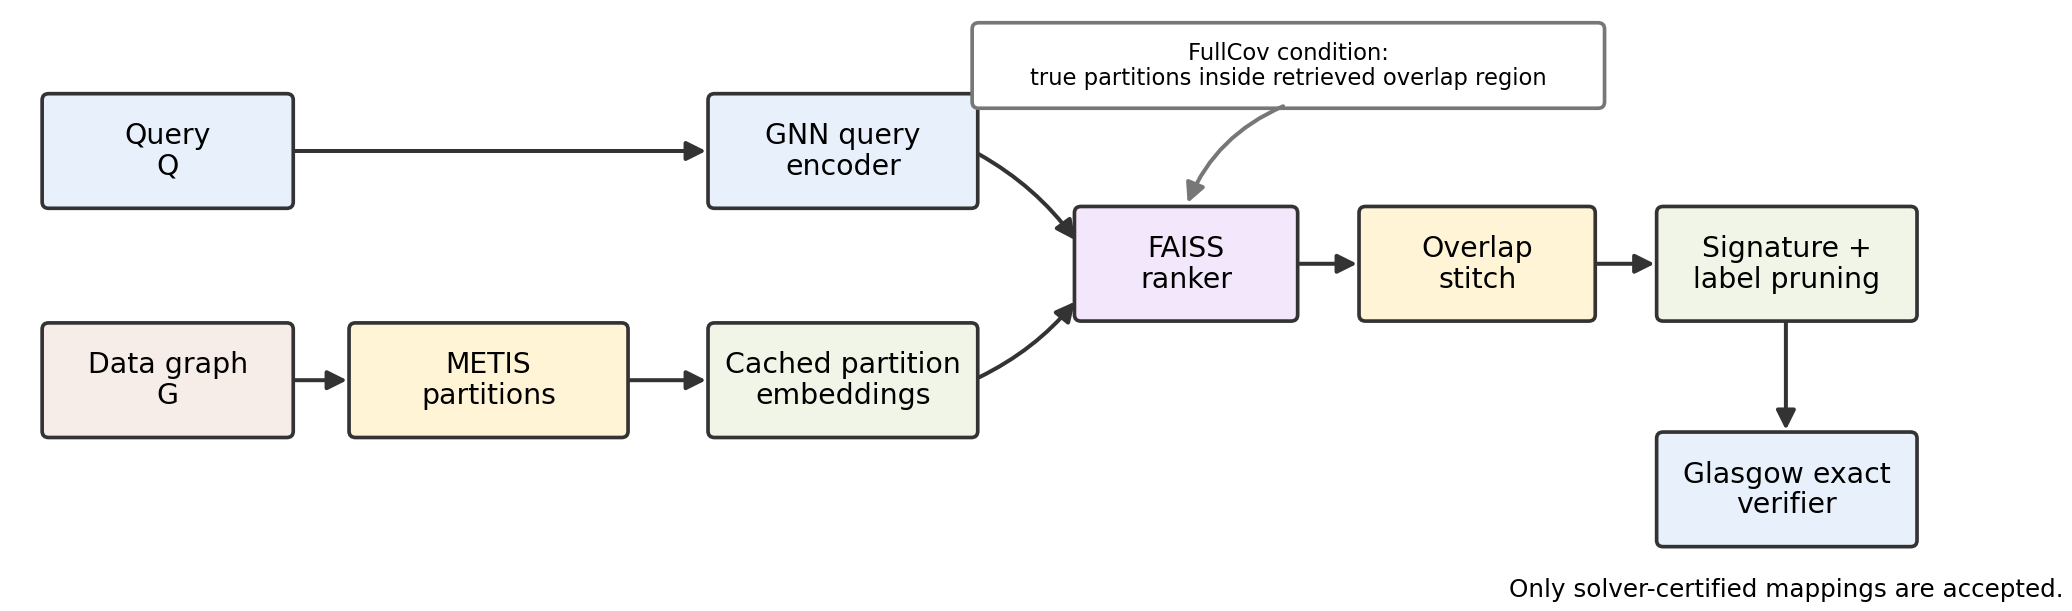
\includegraphics[width=0.78\textwidth]{fig_jigsaw_pipeline.png}
\caption{\textbf{Jigsaw pipeline.} The learned component ranks partitions, but the only accepting step is Glasgow verification inside the stitched candidate graph. FullCov is the condition under which the candidate contains every partition needed by the planted match.}
\label{fig:pipeline}
\end{figure}

\paragraph{Hierarchical localization and overlap cascade.}
The data graph is partitioned into fine and coarse METIS blocks: fine blocks give local structure, coarse blocks are the retrieval units. For each query Jigsaw computes $z_Q=f_\theta(Q)$ and ranks all coarse partitions by cosine similarity to cached partition embeddings (FAISS provides fast top-$K$). True query neighborhoods often cross hard partition boundaries, so Jigsaw stitches the retrieved partitions with one-hop neighboring overlap, increasing recall before verification while still avoiding full-graph search.

\paragraph{Pruning and verification.}
The stitched region is filtered by typed structural signatures (matching coarse type and feature fingerprints) and exact labels (especially important for negative-label queries) before Glasgow verification. Both token sets are derived exclusively from the submitted query payload; planted target-node IDs are evaluation metadata and never enter candidate construction or serving-time pruning. The final answer is produced only by the exact verifier. A shared operator-necessity diagnostic (48 queries per dataset, with metrics over 36 planted positives) is reported at matched half-partition budgets: MAG $K=1{,}000/2{,}000$ and Arxiv $K=100/200$. Removing overlap halves MAG solve rate ($88.9{\to}44.4\%$) and also lowers Arxiv solve rate ($94.4{\to}86.1\%$). Signatures are inert on MAG but control the Arxiv candidate domain: removing them increases mean pruned candidates ${\sim}37\times$ ($76{\to}2{,}815$) without changing solve rate. Thus overlap recovers boundary-crossing matches while signatures prevent candidate explosion on label-rich graphs.

\paragraph{FullCov objective.}
Standard contrastive training rewards high average similarity to positives, which can still leave one required partition ranked too low; Jigsaw optimizes the bottleneck. For query $Q_i$, let $\mathcal{P}_i$ be its positive partitions and $s_{ij}$ the query-partition score. The objective combines multi-positive contrastive learning with a weak-positive term:
\begin{equation}
\mathcal{L}_{\mathrm{weak}}(i)=-\log
\frac{\exp(\min_{p\in\mathcal{P}_i}s_{ip}/\tau)}
{\exp(\min_{p\in\mathcal{P}_i}s_{ip}/\tau)+\sum_{n\in\mathcal{N}_i}\exp(s_{in}/\tau)}.
\end{equation}
Additional CVaR and barrier terms penalize positives below the retrieval budget, and partition embeddings are refreshed from cache with live re-encoding of required positives so the weakest receives a usable gradient. The Arxiv ablation in Table~\ref{tab:loss_ablation} isolates this objective under matched training budgets.

\paragraph{Why the weakest positive.}
The $\min$ (and its CVaR relaxation) follows from the metric. $\mathrm{FullCov@K}(Q)=\mathbf{1}[\mathcal{T}(Q)\subseteq R_K(Q)]$ is a \emph{conjunction}: it succeeds only if \emph{every} $p\in\mathcal{P}_i$ ranks within $K$, so failure is governed by the worst-ranked required partition $\min_{p} s_{ip}$, not the average positive score contrastive learning maximizes. Optimizing the average can raise mean recall while leaving one partition below budget, precisely the failure exact verification cannot tolerate. CVaR (mean of the worst $\alpha$-fraction) is a smooth surrogate for the non-differentiable $\min$, spreading gradient over the hardest positives; hence in Table~\ref{tab:loss_ablation} the objective improves fixed-budget FullCov most at the cascade's operating points, though average recall barely moves.

\subsection{Encoder Architecture and Training Interface}

The encoder is shared between query and partition graphs: features are projected to 256-d, passed through six residual message-passing blocks with LayerNorm, and read out by multi-layer mean/max/sum pooling into an $L_2$-normalized 128-d vector. This matters because the problem is region localization, not node alignment: the model must place a query near \emph{every} partition needed for verification, including the farthest true one. For Cora/Arxiv the block is GraphSAGE~\cite{ref_graphsage} ($\mathtt{SAGEConv}$), at least as strong as GIN at the budgets the cascade uses. OGBN-MAG is \emph{heterogeneous} (paper/author/institution/field nodes, typed relations); we flatten to a single index but \emph{retain} node and relation types via a six-layer RGCN~\cite{ref_rgcn} ($\mathtt{RGCNConv}$, per-relation bases over $2R$ symmetrized relations). Since only paper nodes carry features, others receive node-type one-hot and per-relation-degree features, so the retriever reasons over typed structure.

Both encoders share one retrieval interface: cached fine and coarse partition embeddings are compared to query embeddings, and positive partitions can be live-reencoded during training so coverage gradients update required positives instead of treating the partition bank as stale constants. Training uses three signals: multi-positive contrastive learning toward all touched partitions, hard negatives that separate nearby incorrect partitions, and the FullCov coverage term on the weakest required positive. For MAG, production uses the checkpoint selected by validation FullCov; the final-epoch checkpoint is retained only as a separate diagnostic and is never averaged into production.

\paragraph{Why exactness is conditional.}
The architecture does not make the retriever an exact solver; it proposes a candidate boundary, and once $G_C$ is constructed Glasgow gives exact answers for $G_C$. A positive query can fail for two reasons: the retrieval boundary does not contain the planted solution, or the candidate becomes too large and the solver times out. The benchmark records both through coverage diagnostics, timeout counts, and solved-by-budget curves. Negative queries test whether the candidate construction plus exact verifier returns no match when the generator intended an impossible query.

\section{Experimental Protocol}

\paragraph{Datasets.}
We evaluate Cora~\cite{ref_cora} (small enough for exact timing sanity checks), OGBN-Arxiv~\cite{ref_ogb} (the main medium-scale benchmark), and the full heterogeneous OGBN-MAG (1{,}939{,}743 nodes across four node types joined by typed relations), which stresses the approach with both scale and relation-aware structure and is modeled relation-aware (RGCN over retained node/edge types), not collapsed to an attribute-only homogeneous graph.

\paragraph{Connected-positive protocol.}
All positive families are generated as \emph{connected} planted subgraphs, including the multi-region families.

\paragraph{Label granularity.} The verifier uses discrete labels from hashed full attributes ($\sigma(v)=\mathrm{md5}(x_v)\bmod 10^{6}$), so matches are exact for hashed-label semantics. These highly selective labels make exact-label methods strong and make retrieval mostly a candidate-cost lever; Section~\ref{sec:family} tests coarser $39$-class labels.

\paragraph{Queries and retrieval policies.}
The matrix uses two query seeds, sizes 20/50/100, and 50 queries per type/size/seed. Positives are single, multi-fine, K-hop, degree K-hop, random-walk, and multi-coarse; negatives perturb labels or structure. Policies are learned Jigsaw, MeanFeat, Mean-RRF (reciprocal-rank fusion of the learned Jigsaw and MeanFeat rankings, a configuration of our retriever rather than a nonparametric baseline), TopoFeat, Random, and exhaustive FilterAll.

\paragraph{Partition and overlap scale.}
Tables~\ref{tab:partition_sizes} and~\ref{tab:partition_overlap} summarize the hierarchy. On MAG, a coarse partition has median 969 nodes and borders many partitions, but one-hop overlap admits only boundary nodes (median 4{,}252), not whole neighboring partitions. The union over large budgets can be broad, yet pruning leaves much smaller verifier candidates (Section~\ref{sec:shrinkage}).

\begin{table}[tb]
\centering
\caption{\textbf{Partition balance.} Coarse partitions are ranked by retrieval; fine partitions support local overlap and bridge construction. Node counts are per partition.}
\label{tab:partition_sizes}
\resizebox{\textwidth}{!}{\begin{tabular}{llrrrrrrr}
\toprule
\textbf{Dataset} & \textbf{Level} & \textbf{Graph nodes} & \textbf{Parts} & \textbf{Min} & \textbf{Median} & \textbf{Mean} & \textbf{P90} & \textbf{Max} \\
\midrule
Cora & Coarse & 19,793 & 20 & 962 & 986 & 989.6 & 1,018 & 1,019 \\
Cora & Fine & 19,793 & 100 & 190 & 197 & 197.9 & 204 & 205 \\
Arxiv & Coarse & 169,343 & 200 & 822 & 846 & 846.7 & 872 & 872 \\
Arxiv & Fine & 169,343 & 1,000 & 153 & 169 & 169.3 & 175 & 195 \\
MAG & Coarse & 1,939,743 & 2,000 & 876 & 969 & 969.9 & 999 & 999 \\
MAG & Fine & 1,939,743 & 10,000 & 170 & 194 & 194.0 & 200 & 210 \\
\bottomrule
\end{tabular}
}
\end{table}

\begin{table}[tb]
\centering
\caption{\textbf{Overlap expansion scale.} The operator adds boundary nodes of edge-sharing partitions, not whole neighboring partitions; the loose union bound is never materialized.}
\label{tab:partition_overlap}
\footnotesize
\resizebox{\textwidth}{!}{\begin{tabular}{lrrrrrr}
\toprule
\textbf{Dataset} & \textbf{Coarse parts} & \shortstack{\textbf{Partition}\\\textbf{nodes (med)}} & \shortstack{\textbf{+Boundary}\\\textbf{overlap (med)}} & \shortstack{\textbf{Expanded part}\\\textbf{(med / $\times$)}} & \shortstack{\textbf{Neighbor parts}\\\textbf{med / max}} & \shortstack{\textbf{Loose union}\\\textbf{bound (med)}} \\
\midrule
Cora  & 20    & 986 & 534   & 1,533 / 1.6$\times$ & 18 / 19    & 18,820 \\
Arxiv & 200   & 846 & 1,606 & 2,470 / 2.9$\times$ & 135 / 173  & 115,004 \\
MAG   & 2,000 & 969 & 4,252 & 5,228 / 5.4$\times$ & 948 / 1,999 & 921,494 \\
\bottomrule
\end{tabular}
}
\end{table}

\paragraph{Metrics.}
We report FullCov@K/recall for retrieval and exact-solve rate, no-match accuracy, false positives, timeouts, candidate size, and wall-clock components for verification.

\paragraph{Benchmark completion and data hygiene.}
Each dataset has 2,400 unique queries: 1,800 positives (6 families) and 600 negatives (2 families), from 2 seeds, 3 sizes, and 50 queries per cell. Applying 6 policies gives 14,400 policy-query evaluations before budget expansion, summarized by 288 production rows (6 methods $\times$ 2 seeds $\times$ 8 families $\times$ 3 sizes). A serving-path audit covers all 7,200 unique queries: query-payload tokens equal the legacy evaluation tokens for all 5,400 positives, all 900 label-corrupted negatives intentionally diverge, and all 1,800 negatives were rerun with pruning tokens derived only from each submitted query. Diagnostic variants are kept separate from canonical rows.

\paragraph{Implementation.} Partitioning uses METIS, embeddings use FAISS, and Glasgow verifies integer-labeled candidates obtained by discretizing node features. Timings are per-query wall-clock on 8-vCPU Google Cloud instances with a 30\,s verifier budget. Encoders, query seeds, hierarchies, and manifests will be released.

\section{Results}

\subsection{FullCov Training Improves Retrieval}

Table~\ref{tab:loss_ablation} gives the matched-budget Arxiv retrieval result. All rows use the same locked K-hop query seeds and 9,000 optimizer steps. The FullCov objective improves the fixed-budget operating points most relevant to bounded exact verification.

\begin{table}[H]
\centering
\caption{\textbf{Matched Arxiv retrieval objective ablation.} Fixed retrieval budgets on $n{=}400$ locked K-hop queries (200 per query seed); each row averages the validation-selected checkpoint from two independent training replicates.}
\label{tab:loss_ablation}
\small
\setlength{\tabcolsep}{5pt}
\resizebox{\textwidth}{!}{%
\begin{tabular}{lcccc}
\toprule
\textbf{Objective} & \textbf{FullCov@20} & \textbf{FullCov@50} & \textbf{FullCov@100} & \textbf{Mean worst rank} \\
\midrule
Contrastive control & 21.7\% & 39.0\% & 66.0\% & 74.02 \\
FullCov objective & \textbf{26.0\%} & \textbf{48.8\%} & \textbf{82.0\%} & \textbf{58.97} \\
\midrule
McNemar $p$ & $4.6{\times}10^{-3}$ & $9.8{\times}10^{-6}$ & $4.0{\times}10^{-10}$ & -- \\
\bottomrule
\end{tabular}}
\end{table}

The locked K-hop suite has zero queries impossible at $K=20,50,100$; average true coarse footprint is 6.37 and maximum footprint is 17. The objective therefore improves ranking by explicitly optimizing the weakest required partition. Because the control and FullCov-aligned models share query seeds and training budget, the gain comes from the objective rather than easier queries or longer optimization. The largest improvement appears at FullCov@100, where the downstream verifier has enough room to benefit from better ordering without searching the whole graph, exactly the cascade's operating point.

\clearpage
\begin{samepage}
\subsection{Three-Dataset Production Matrix}

Table~\ref{tab:production_matrix} reports exact planted-match recovery, correct no-match behavior, false positives, solver timeouts, candidate nodes, cascade time, and verifier time. Cascade time sums candidate construction and exact verification and excludes retrieval/ranking.
\end{samepage}

\begin{table}[H]
\centering
\caption{\textbf{Final production metrics.} Pos. uses matched half-partition budgets $K{=}10/100/1000$; FilterAll uses the all-partition ceiling. Neg. is audited no-match accuracy; FP counts negative false positives, while TO counts positive-query solver timeouts (FeatureIndex was run on positives only). Candidate and timing columns use the same endpoint as Pos. Cascade time is candidate construction plus exact verification and excludes retrieval/ranking.}
\label{tab:production_matrix}
\setlength{\tabcolsep}{2.5pt}
\resizebox{\textwidth}{!}{%
\begin{tabular}{llrrrrrrr}
\toprule
\textbf{Dataset} & \textbf{Method} & \textbf{Pos. \%} & \textbf{Neg. \%} & \textbf{FP} & \textbf{TO} & \textbf{Cand. nodes} & \textbf{Cascade s} & \textbf{Solver ms} \\
\midrule
Cora & Jigsaw & 94.2 & 100.0 & 0 & 0 & 458 & 0.05 & 11.8 \\
Cora & Mean-RRF & 93.8 & 100.0 & 0 & 0 & 485 & 0.05 & 11.8 \\
Cora & MeanFeat & 87.7 & 100.0 & 0 & 0 & 1.13K & 0.06 & 10.5 \\
Cora & TopoFeat & 31.9 & 100.0 & 0 & 0 & 7.60K & 0.17 & 3.6 \\
Cora & Random & 32.7 & 100.0 & 0 & 0 & 7.54K & 0.16 & 3.8 \\
Cora & FilterAll$^\ddagger$ & 100.0 & 100.0 & 0 & 0 & 59 & 0.06 & 12.7 \\
\midrule
Arxiv & Jigsaw & 92.8 & 100.0 & 0 & 0 & 77 & 0.19 & 18.3 \\
Arxiv & Mean-RRF & 94.0 & 100.0 & 0 & 0 & 75 & 0.19 & 18.8 \\
Arxiv & MeanFeat & 89.7 & 100.0 & 0 & 0 & 91 & 0.22 & 18.4 \\
Arxiv & TopoFeat & 33.3 & 100.0 & 0 & 0 & 233 & 0.46 & 6.0 \\
Arxiv & Random & 39.2 & 100.0 & 0 & 0 & 219 & 0.47 & 7.0 \\
Arxiv & FilterAll$^\ddagger$ & 100.0 & 100.0 & 0 & 0 & 57 & 0.35 & 19.1 \\
\midrule
MAG & Jigsaw & \textbf{88.6} & 99.5 & 1 & 25 & 138.1K & 6.97 & 81.9 \\
MAG & Mean-RRF & 85.4 & 99.5 & 1 & 17 & 137.1K & 5.38 & 67.9 \\
MAG & FeatureIndex$^\S$ & \textbf{96.7} & -- & -- & 24 & 59.4K & 2.39 & 118.8 \\
MAG & MeanFeat & 64.6 & 99.5 & 1 & 12 & 212.1K & 8.02 & 27.5 \\
MAG & TopoFeat & 37.1 & 99.8 & 1 & 1 & 235.6K & 8.07 & 5.2 \\
MAG & Random & 51.4 & 99.7 & 1 & 9 & 282.1K & 9.54 & 19.9 \\
MAG & FilterAll$^\ddagger$ & 98.4 & 99.3 & 1 & 33 & 443.8K & 5.85 & 288.6 \\
\bottomrule
\end{tabular}}
\end{table}

At the half-partition budget (Table~\ref{tab:production_matrix}) Jigsaw solves $94.2/92.8/88.6\%$ on Cora/Arxiv/MAG. The $100\%$ Cora/Arxiv entries are the exhaustive ceiling, not a retrieval result; Mean-RRF is competitive there, and FeatureIndex is strongest on MAG under near-unique labels. Matched Cora/Arxiv costs are now measured for every policy: Jigsaw uses mean terminal candidates 458/77, cascade times 0.05/0.19\,s, and verifier times 11.8/18.3\,ms. Size 100 is harder (Cora $89.0\%$ vs. $96.8/96.8\%$ at 20/50; Arxiv $90.3\%$ vs. $93.8/94.2\%$), driven by Cora random-walk ($75.3\%$) and Arxiv multi-coarse ($78.7\%$). On MAG, recovery declines from $93.2\%$ at size 20 to $90.7\%$ at 50 and $82.0\%$ at 100, driven by random-walk ($94/100$, $79/100$, $40/100$), while contained multi-fine remains perfect at every size and multi-coarse remains difficult ($77/100$, $79/100$, $72/100$). Jigsaw sends fewer candidate nodes than FilterAll (138K vs 444K) and has lower verifier time (82 vs 289 ms), while FilterAll remains the recall ceiling at 98.4\%. The cascade also streams the graph: partition-wise pruning before edge materialization peaks at \textbf{2.4\,GB} on a 54-query MAG grid (6 families $\times$ 3 sizes $\times$ 3 queries) versus \textbf{10.2\,GB} for whole-graph residence ($4.2\times$), recovering $46/54$ matches.

\paragraph{Label-selectivity crossover.} Near-unique md5 labels favor exact-label methods: a classical label-coverage index (\textbf{FeatureIndex}, in the GraphGrep~\cite{ref_graphgrep}/gIndex~\cite{ref_gindex} tradition) is the strongest bounded retriever here ($96.7\%$; median worst-true-partition rank $104$ of $2{,}000$) versus the learned GNN ($88.6\%$; rank ${\sim}900$). At coarse $39$-class labels this ranking order \emph{inverts}: the learned model has better worst-true-partition ranks in each family, while complete solve runs are statistically tied (FeatureIndex $63.4\%$; learned variants $63$--$64\%$). This isolates the regime in which learning contributes: as labels stop localizing, the GNN supplies the better partition ranking. Spatially extended families remain the hardest because FullCov must recover all $16$--$30$ touched partitions. Inference-time probes shift their coverage by at most ${\approx}{+}2.3$ points, while the high-degree partition graph explains why broad neighborhood aggregation cannot selectively trace the query footprint. These results make representation-level footprint coverage the next learning target. The crossover generalizes on Cora and Arxiv, where the winner flips with an offline label-selectivity statistic (median partitions/label $1$ at feature labels versus $12$/$124.5$ at class labels), allowing Jigsaw to select its bounded retriever by label regime (Table~\ref{tab:selectivity_xd_ecml}). Jigsaw is therefore \emph{retriever-agnostic}, while FullCov and coarse-label localization establish that learning is an essential operating regime of the system.

\begin{table}[H]
\centering
\caption{Cross-dataset label-selectivity crossover: overall median worst-true-partition rank (lower is better; retrieval-only, $n{=}540$ per dataset = 2 seeds $\times$ 6 positive families $\times$ 3 sizes $\times$ 15 queries). Near-unique feature labels favor the classical index; realistic class labels favor the learned retriever. MAG shows the same inversion at scale.}
\label{tab:selectivity_xd_ecml}
\small
\begin{tabular}{lcccc}
\toprule
 & \multicolumn{2}{c}{FeatureIndex} & Learned & Parts/label \\
\cmidrule(lr){2-3}
Dataset (parts) & feature & class & (any) & feat / class \\
\midrule
Cora ($20$)   & 2 & 7   & 5  & $1$ / $12$ \\
Arxiv ($200$) & 4 & 104 & 44 & $1$ / $124.5$ \\
\bottomrule
\end{tabular}
\end{table}

The central systems result is the scaling break: direct CP-based Glasgow solves all 15 Cora K-hop queries but \textbf{0 of 15} on Arxiv and MAG, whereas the Jigsaw cascade remains feasible by handing the verifier a small candidate. The retriever therefore sits on a recall--cost frontier: FeatureIndex is strongest under near-unique MAG labels, FilterAll is the exhaustive ceiling, and the learned retriever is a useful memory-bounded point, especially once labels coarsen.

\begin{figure}[H]
\centering
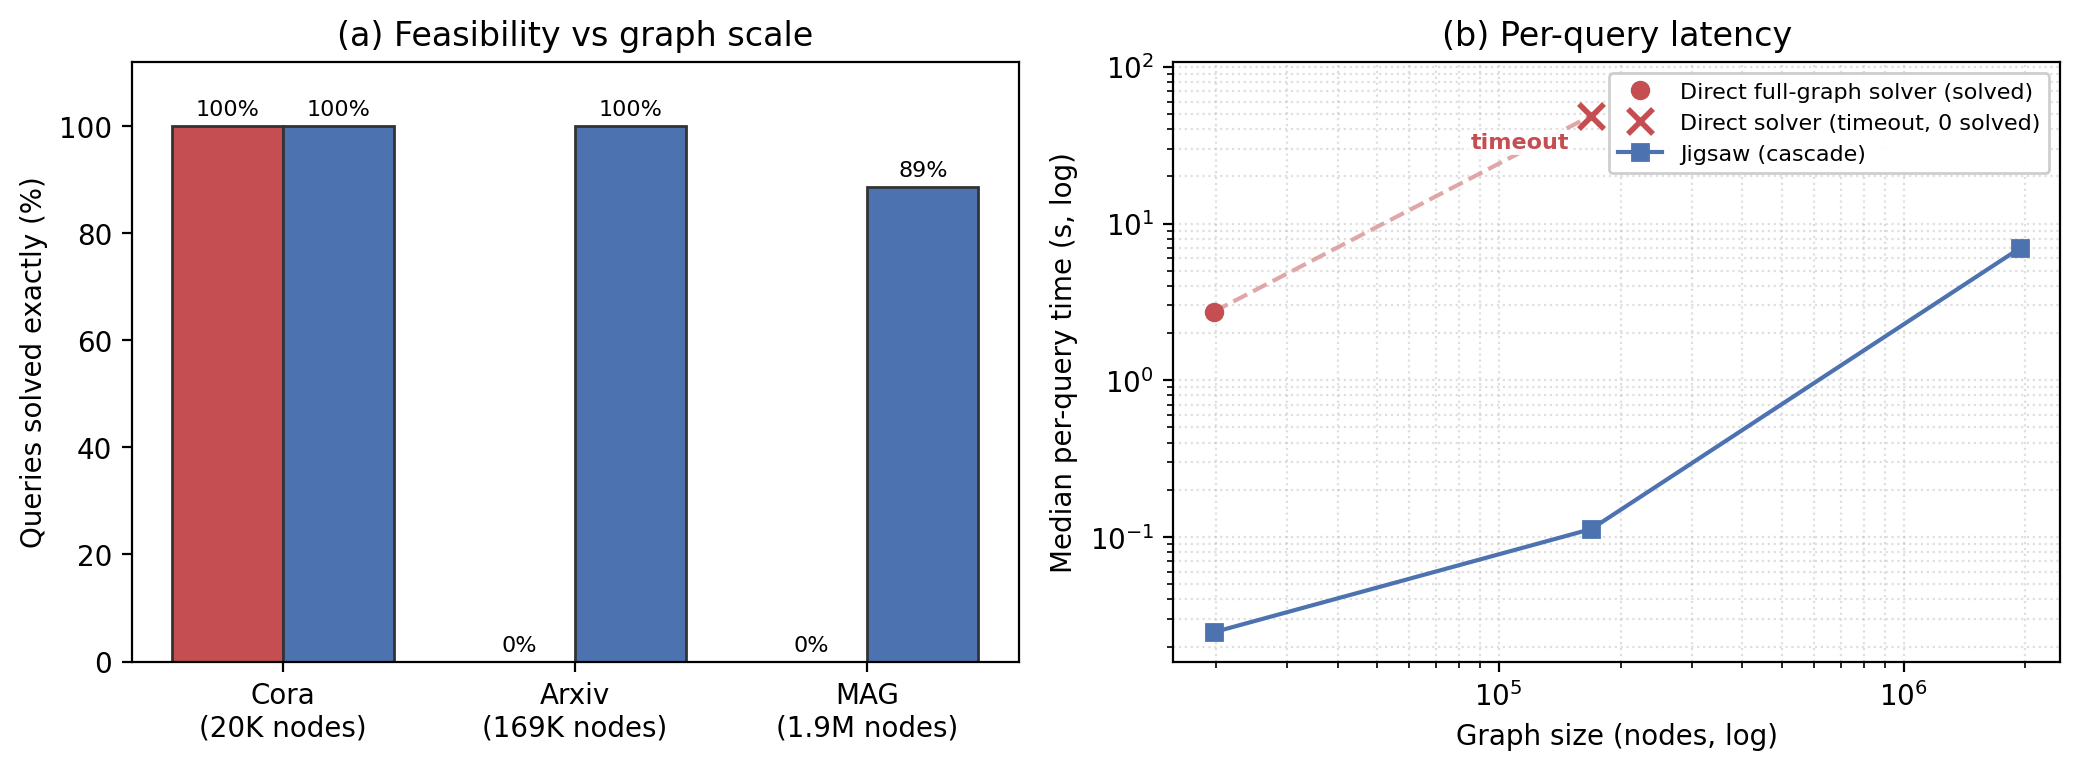
\includegraphics[width=0.82\textwidth]{fig_scaling_feasibility.png}
\caption{\textbf{Jigsaw makes the exact solver's domain tractable.} Direct full-graph Glasgow solves Cora but none of the Arxiv/MAG K-hop samples; Jigsaw stays feasible by verifying only the retrieved-and-pruned candidate.}
\label{fig:scaling}
\end{figure}

\begin{table}[H]
\centering
\caption{\textbf{Scaling and latency: direct full-graph solver vs.\ Jigsaw cascade.} Cora/Arxiv use the same 15 K-hop queries and Jigsaw is evaluated at matched half-partition budgets ($K=10/100$), avoiding exhaustive Cora retrieval. The MAG direct cell is its 15-query timeout diagnostic, while $^\ast$ the MAG Jigsaw cell is separately the 1,800-positive production mean at $K=1{,}000$.}
\label{tab:scaling_latency}
\small
\begin{tabular}{l r c r c r r}
\toprule
 & & \multicolumn{2}{c}{Direct full-graph solver} & \multicolumn{2}{c}{Jigsaw cascade} & Cand.\ \\
\cmidrule(lr){3-4}\cmidrule(lr){5-6}
Dataset & Nodes & Solved & Med.\ time & Solved & Med.\ time & nodes \\
\midrule
Cora  & 19.8K & 15/15 & $2.74$\,s & 15/15 & $\mathbf{0.03}$\,s & 50 \\
Arxiv & 169K  & \textbf{0/15}$^\dagger$ & ${\approx}49$\,s & 15/15 & $\mathbf{0.11}$\,s & 50 \\
MAG   & 1.9M  & \textbf{0/15} & timeout & 88.6\% & $6.97$\,s$^\ast$ & -- \\
\bottomrule
\end{tabular}
\end{table}

\paragraph{Statistical significance.}
Table~\ref{tab:significance} reports bootstrap confidence intervals and paired exact-McNemar tests for MAG positives. Jigsaw significantly beats the learned/feature retrievers except FilterAll, which is the exhaustive ceiling. These are component comparisons; the system contribution is exact matching without whole-graph residence and with fewer candidates than FilterAll.

\begin{table}[H]
\centering
\caption{\textbf{MAG solve-rate significance.} Bootstrap 95\% CI over $n{=}1800$ positive queries, and paired exact-McNemar of Jigsaw vs each policy (wins = queries Jigsaw solves and the other does not).}
\label{tab:significance}
\small
\setlength{\tabcolsep}{6pt}
\begin{tabular}{lccc}
\toprule
\textbf{Method} & \textbf{Solve \%} & \textbf{95\% CI} & \textbf{vs Jigsaw (W/L, $p$)} \\
\midrule
Jigsaw    & 88.6 & [87.1, 90.0] & -- \\
Mean-RRF  & 85.4 & [83.7, 87.0] & 92 / 35, \ $p{=}4.4{\times}10^{-7}$ \\
MeanFeat  & 64.6 & [62.3, 66.8] & 437 / 51, \ $p{<}10^{-76}$ \\
Random    & 51.4 & [49.1, 53.8] & 689 / 67, \ $p{<}10^{-130}$ \\
Topo      & 37.1 & [34.9, 39.5] & 912 / 32, \ $p{<}10^{-224}$ \\
FilterAll & 98.4 & [97.8, 98.9] & 2 / 225, \ $p{=}2.4{\times}10^{-64}$ \\
\bottomrule
\end{tabular}
\end{table}

\begin{table}[H]
\centering
\caption{\textbf{Jigsaw query-family breakdown.} Positive columns report exact-solve rate; negative columns report correct no-match rate. All three datasets use the connected-positive protocol. All datasets are reported at the matched half-partition budget ($K{=}10/100/1000$); the MAG rows use the deployed walk-aware encoder (overall $88.6\%$).}
\label{tab:jigsaw_family}
\setlength{\tabcolsep}{3pt}
\resizebox{\textwidth}{!}{%
\begin{tabular}{lrrrrrrrr}
\toprule
\textbf{Dataset} & \textbf{Single} & \textbf{K-hop} & \textbf{Deg-K} & \textbf{Walk} & \textbf{Multi-fine} & \textbf{Multi-coarse} & \textbf{Neg-label} & \textbf{Neg-struct} \\
\midrule
Cora & 100.0 & 98.3 & 97.3 & 75.3 & 100.0 & 94.3 & 100.0 & 100.0 \\
Arxiv & 100.0 & 97.3 & 98.3 & 82.3 & 100.0 & 78.7 & 100.0 & 100.0 \\
MAG & 98.7 & 93.3 & 92.7 & 71.0 & 100.0 & 76.0 & 100.0 & 99.0 \\
\bottomrule
\end{tabular}}
\end{table}

\label{sec:family}
The family view explains the aggregate rates. Single and multi-fine saturate, local K-hop families remain high, and random-walk/multi-coarse are hardest across datasets. MAG still solves single $98.7\%$, K-hop $93.3\%$, degree K-hop $92.7\%$, and multi-fine $100\%$; random walks remain lowest at $71.0\%$.

Random walks provide the main stress test. FilterAll solves them at $96.0\%$, and $96.6\%$ of Jigsaw's random-walk misses occur before solving, locating the opportunity in retrieval and overlap coverage rather than Glasgow. Compact K-hop misses often lie on retrieved boundaries and overlap repairs them; diffuse walk misses more often lie in unretrieved interiors. The held-out walk-aware encoder lifts random-walk $60.0\%\!\to\!71.0\%$ and multi-coarse $71.7\%\!\to\!76.0\%$ relative to the generic encoder, showing that learning improves the families in which spatial coverage matters most.

Cumulative solved-by-budget curves rise monotonically to $94.2/92.8/88.6$ at the half-partition budget. On MAG, solve rate rises from $37.6\%$ at small budgets to $88.6\%$ at $K{=}1000$, confirming that candidate coverage, rather than verifier soundness, controls the budget frontier.

\subsection{Candidate-Shrinkage Cascade and Boundary Overlap}
\label{sec:shrinkage}

A natural objection is that one-hop overlap might expand to most of the graph. We test the per-query cascade
\[
\text{full graph} \to \text{overlap} \to \text{signature} \to \text{label-pruned} \to \text{solver components},
\]
on 14{,}400 positive method/model-query evaluation records over the 1{,}800-query MAG positive grid. Hybrid and Mean-RRF each contribute two model variants; this is not a unique-query denominator. Three facts emerge.

\textbf{(1) Overlap is broad, but ranking still removes most of the graph.} The median selected-overlap union is 59\% of MAG for Jigsaw, yet after identical pruning the candidate is 84.5K nodes versus 544K for FilterAll, a $6.4\times$ median reduction.

\textbf{(2) Pruning is coverage-lossless.} Recall loss occurs at retrieval/overlap, not attribute pruning:

\begin{proposition}[Lossless pruning]
\label{prop:lossless}
Let the pruning token $\sigma(\cdot)$ be a node attribute that the matching semantics preserve, i.e.\ any valid embedding $\phi$ of $Q$ into $G$ satisfies $\sigma(\phi(q))=\sigma(q)$ for every query node $q$ (vertex-labelled matching, with $\sigma$ derived from node type and feature labels). Prune the candidate $G_C$ to $G_C'=\{v\in G_C : \sigma(v)\in \sigma(V_Q)\}$. Then for any embedding $\phi$ with $\phi(V_Q)\subseteq G_C$, we have $\phi(V_Q)\subseteq G_C'$. Hence pruning preserves node coverage: $\mathrm{FullCov}$ is unchanged.
\end{proposition}
\emph{Proof.} For $q\in V_Q$, $\sigma(\phi(q))=\sigma(q)\in\sigma(V_Q)$, so $\phi(q)$ satisfies the keep condition and is retained. Thus every matched node survives.

\begin{samepage}
The cascade signatures and exact-label filters are attribute invariants, so the proposition applies. Empirically, planted-match survival after overlap equals survival after pruning for every policy (Jigsaw $87\%$ both), so the solve ceiling is set by whether the retrieved-plus-overlapped region contains the match.
\end{samepage}

\textbf{(3) Candidate construction dominates latency:} mean build is $3.4$\,s for Jigsaw and $5.5$\,s for FilterAll versus $0.25$\,s of solving.

\paragraph{Boundary overlap is an essential recall operator.}
The matched ablation shows the effect directly: removing boundary overlap cuts solve rate from $88.9\%$ to $44.4\%$ on MAG and from $94.4\%$ to $86.1\%$ on Arxiv. Its benefit is strongest for compact local structure. Boundary expansion recovers missed true partitions for $94\%$ of K-hop queries but for $62\%$ of random-walk queries, whose matches more often extend into the interior of an unselected partition. Together with coverage-lossless pruning, this locates the remaining errors before verification, when retrieval plus boundary overlap does not cover the match.

\subsection{What the Ablations Establish}

The ablations show why the cascade needs multiple operators. At matched half-partition budgets, removing overlap lowers positive solve rate from $88.9$ to $44.4\%$ on MAG and from $94.4$ to $86.1\%$ on Arxiv. Removing signatures leaves Arxiv solve rate unchanged but expands mean pruned candidates ${\sim}37\times$ ($76\to2{,}815$). Exact-label pruning and component decomposition remain important on MAG ($88.9\to52.8\%$ and $88.9\to63.9\%$ when removed).

Diagnostic variants are kept separate from the canonical validation-selected matrix.

\subsection{Negative Queries and Soundness}

Jigsaw never accepts from the neural model alone; Glasgow is the only accepting step. Audited no-match accuracy is 100.0\% for Cora/Arxiv and 99.3--99.8\% across MAG policies, with at most one false positive per method; the remaining errors are timeout/unknown outcomes. The rare false positives are benchmark-level failures, not verifier hallucinations: a returned mapping is a true isomorphism inside the candidate, but a perturbed ``negative'' may still match elsewhere. The reported metric is audited no-match accuracy under this synthetic protocol; global non-existence would require exhaustive full-graph certification.

\section{Discussion and Limitations}
\label{sec:limits}

Jigsaw is an exact-verification system with a learned search boundary. Retrieval coverage controls completeness, while Glasgow preserves sound acceptance inside every candidate; FullCov makes that boundary measurable and trainable. The design targets static attributed graphs and repeated query workloads where partitioning, embeddings, and FAISS indexes amortize. FeatureIndex leads under near-unique labels, and learned retrieval becomes the better localizer as labels coarsen.

\paragraph{Evaluation scope.} We compare against feature/structure index rankers, no-retrieval Glasgow, exhaustive FilterAll, uninformed retrievers, and scalable CFL-Match/DP-iso/GQL controls. These controls locate Jigsaw's advantage in CP-based Glasgow service, bounded residence, and low-selectivity candidate construction. NeuroMatch and GLSearch use released protocols for smaller contained-query targets rather than a partitioned million-node path. Out-of-core and distributed matchers stream or shard the entire graph; Jigsaw exposes a complementary single-machine frontier by paying one-time partitioning and indexing cost to bound residence by learned relevance. The benchmark uses planted connected subgraphs on static graphs, and the label-coarsening experiments explicitly isolate the weak-label regime where learned localization contributes.

\section{Conclusion}

Jigsaw turns learned graph retrieval into an execution mechanism for exact search: ML predicts which regions deserve memory and verification, while Glasgow remains the sole accepting authority. On full MAG this changes the tested operating point from 0/15 direct CP solves to 88.6\% exact positive recovery with the learned retriever, while streaming at 2.4\,GB instead of 10.2\,GB for whole-graph residence. FullCov aligns learning with the decisive failure event of missing even one required partition, while overlap and lossless pruning make the verifier usable under bounded memory. A resident exact solver dominates when selective labels collapse its candidate tables; under weak labels, whole-graph candidate construction fails and Jigsaw's bounded candidate supplies the relevant systems advantage. FullCov improves fixed-budget coverage, and after label coarsening the learned ranker localizes required partitions better than the classical label index, although their end-to-end coarse-label solve rates remain tied. Jigsaw is therefore \emph{retriever-agnostic} by construction, choosing a classical index under near-unique labels and learned ranking when labels cease to localize. The result is exact subgraph verification made usable on million-node graphs without replacing exactness by a neural guess. The inference-time probes further locate diffuse-query errors in representation-level coverage, providing a concrete direction for the learned component.

\paragraph{Use of Generative AI.}
Generative AI tools assisted with language editing and software scaffolding; all research design, experiments, analyses, and claims are the authors' own.

\begin{thebibliography}{39}

\bibitem{ref_glasgow}
McCreesh, C., Prosser, P., Trimble, J.: The Glasgow Subgraph Solver: Using Constraint Programming to Tackle Hard Subgraph Isomorphism Problem Variants. In: CP 2020 (2020)

\bibitem{ref_gin}
Xu, K., Hu, W., Leskovec, J., Jegelka, S.: How Powerful are Graph Neural Networks? In: ICLR (2019)

\bibitem{ref_graphsage}
Hamilton, W.L., Ying, R., Leskovec, J.: Inductive Representation Learning on Large Graphs. In: NeurIPS, pp. 1024--1034 (2017)

\bibitem{ref_rgcn}
Schlichtkrull, M., Kipf, T.N., Bloem, P., van den Berg, R., Titov, I., Welling, M.: Modeling Relational Data with Graph Convolutional Networks. In: ESWC, pp. 593--607 (2018)

\bibitem{ref_vf2}
Cordella, L.P., Foggia, P., Sansone, C., Vento, M.: A (Sub)Graph Isomorphism Algorithm for Matching Large Graphs. IEEE TPAMI \textbf{26}(10), 1367--1372 (2004)

\bibitem{ref_faiss}
Johnson, J., Douze, M., J\'egou, H.: Billion-Scale Similarity Search with GPUs. IEEE Trans. Big Data \textbf{7}(2), 535--547 (2021)

\bibitem{ref_metis}
Karypis, G., Kumar, V.: A Fast and High Quality Multilevel Scheme for Partitioning Irregular Graphs. SIAM J. Sci. Comput. \textbf{20}(1), 359--392 (1998)

\bibitem{ref_ogb}
Hu, W., et al.: Open Graph Benchmark: Datasets for Machine Learning on Graphs. In: NeurIPS (2020)

\bibitem{ref_garey}
Garey, M.R., Johnson, D.S.: Computers and Intractability: A Guide to the Theory of NP-Completeness. W.H. Freeman (1979)

\bibitem{ref_ullmann}
Ullmann, J.R.: An Algorithm for Subgraph Isomorphism. J. ACM \textbf{23}(1), 31--42 (1976)

\bibitem{ref_ri}
Bonnici, V., Giugno, R., Pulvirenti, A., Shasha, D., Ferro, A.: A Subgraph Isomorphism Algorithm and Its Application to Biochemical Data. BMC Bioinformatics \textbf{14}(Suppl 7), S13 (2013)

\bibitem{ref_lad}
Solnon, C.: AllDifferent-Based Filtering for Subgraph Isomorphism. Artificial Intelligence \textbf{174}(12--13), 850--864 (2010)

\bibitem{ref_cora}
Sen, P., Namata, G., Bilgic, M., Getoor, L., Galligher, B., Eliassi-Rad, T.: Collective Classification in Network Data. AI Magazine \textbf{29}(3), 93--106 (2008)

\bibitem{ref_neuromatch}
Ying, R., et al.: Neural Subgraph Matching. arXiv:2007.03092 (2020)

\bibitem{ref_gnnpe}
Ye, Y., Lian, X., Chen, M.: Efficient Exact Subgraph Matching via GNN-based Path Dominance Embedding. Proc. VLDB Endow. \textbf{17}(7), 1628--1641 (2024)

\bibitem{ref_glsearch}
Liu, Y., et al.: GLSearch: Maximum Common Subgraph Detection via Learning to Search. In: ICML (2021)

\bibitem{ref_nsic}
Liu, X., Pan, H., He, M., Song, Y., Jiang, X., Shang, L.: Neural Subgraph Isomorphism Counting. In: KDD (2020)

\bibitem{ref_turboiso}
Han, W.S., Lee, J., Lee, J.H.: TurboISO: Towards Ultrafast and Robust Subgraph Isomorphism Search in Large Graph Databases. In: SIGMOD (2013)

\bibitem{ref_cflmatch}
Bi, F., Chang, L., Lin, X., Qin, L., Zhang, W.: Efficient Subgraph Matching by Postponing Cartesian Products. In: SIGMOD (2016)

\bibitem{ref_daf}
Han, M., Kim, H., Gu, G., Park, K., Han, W.S.: Efficient Subgraph Matching: Harmonizing Dynamic Programming, Adaptive Matching Order, and Failing Set Together. In: SIGMOD (2019)

\bibitem{ref_graphql}
He, H., Singh, A.K.: Graphs-at-a-Time: Query Language and Access Methods for Graph Databases. In: SIGMOD, pp. 405--418 (2008)

\bibitem{ref_vf3}
Carletti, V., Foggia, P., Saggese, A., Vento, M.: Challenging the Time Complexity of Exact Subgraph Isomorphism for Huge and Dense Graphs with VF3. IEEE Trans. Pattern Anal. Mach. Intell. \textbf{40}(4), 804--818 (2018)

\bibitem{ref_gsi}
Zeng, L., Zou, L., \"{O}zsu, M.T., Hu, L., Zhang, F.: GSI: GPU-friendly Subgraph Isomorphism. In: ICDE, pp. 1249--1260 (2020)

\bibitem{ref_survey}
Sun, S., Luo, Q.: In-Memory Subgraph Matching: An In-depth Study. In: SIGMOD (2020)

\bibitem{ref_survey2024}
Zhang, Z., Lu, Y., Zheng, W., Lin, X.: A Comprehensive Survey and Experimental Study of Subgraph Matching: Trends, Unbiasedness, and Interaction. Proc. ACM Manag. Data \textbf{2}(1), Article 60 (2024)

\bibitem{ref_wcoj}
Mhedhbi, A., Salihoglu, S.: Optimizing Subgraph Queries by Combining Binary and Worst-Case Optimal Joins. Proc. VLDB Endow. \textbf{12}(11), 1692--1704 (2019)

\bibitem{ref_lowmem}
Ammar, K., McSherry, F., Salihoglu, S., Joglekar, M.: Distributed Evaluation of Subgraph Queries Using Worst-Case Optimal Low-Memory Dataflows. Proc. VLDB Endow. \textbf{11}(6), 691--704 (2018)

\bibitem{ref_dualsim}
Kim, H., Lee, J., Bhowmick, S.S., Han, W.-S., Lee, J., Ko, S., Jarrah, M.H.A.: DUALSIM: Parallel Subgraph Enumeration in a Massive Graph on a Single Machine. In: SIGMOD (2016)

\bibitem{ref_trinity}
Sun, Z., Wang, H., Wang, H., Shao, B., Li, J.: Efficient Subgraph Matching on Billion Node Graphs. Proc. VLDB Endow. \textbf{5}(9), 788--799 (2012)

\bibitem{ref_gthinker}
Yan, D., Guo, G., Chowdhury, M.M.R., \"{O}zsu, M.T., Ku, W.-S., Lui, J.C.S.: G-thinker: A Distributed Framework for Finding Qualified Subgraphs in a Big Graph with Load Balancing. In: ICDE (2020)

\bibitem{ref_simgnn}
Bai, Y., Ding, H., Bian, S., Chen, T., Sun, Y., Wang, W.: SimGNN: A Neural Network Approach to Fast Graph Similarity Computation. In: WSDM, pp. 384--392 (2019)

\bibitem{ref_gmn}
Li, Y., Gu, C., Dullien, T., Vinyals, O., Kohli, P.: Graph Matching Networks for Learning the Similarity of Graph Structured Objects. In: ICML, PMLR \textbf{97}, 3835--3845 (2019)

\bibitem{ref_psimgnn}
Xu, H., Duan, Z., Wang, Y., Feng, J., Chen, R., Zhang, Q., Xu, Z.: Graph Partitioning and Graph Neural Network Based Hierarchical Graph Matching for Graph Similarity Computation. Neurocomputing \textbf{439}, 348--362 (2021)

\bibitem{ref_isonet}
Roy, I., Velugoti, V.S.B.R., Chakrabarti, S., De, A.: Interpretable Neural Subgraph Matching for Graph Retrieval. In: AAAI \textbf{36}(7), 8115--8123 (2022)

\bibitem{ref_isonetpp}
Ramachandran, A., Raj, V., Roy, I., Chakrabarti, S., De, A.: Iteratively Refined Early Interaction Alignment for Subgraph Matching Based Graph Retrieval. In: NeurIPS \textbf{37} (2024)

\bibitem{ref_neuraldesign}
Raj, V., Roy, I., Ramachandran, A., Chakrabarti, S., De, A.: Charting the Design Space of Neural Graph Representations for Subgraph Matching. In: ICLR (2025)

\bibitem{ref_neugn}
Ying, Y., Dai, Y., Li, W., et al.: Neural Graph Navigation for Intelligent Subgraph Matching. In: AAAI \textbf{40}(19), 16181--16189 (2026)

\bibitem{ref_graphgrep}
Shasha, D., Wang, J.T.L., Giugno, R.: Algorithmics and Applications of Tree and Graph Searching. In: PODS, pp. 39--52 (2002)

\bibitem{ref_gindex}
Yan, X., Yu, P.S., Han, J.: Graph Indexing: A Frequent Structure-based Approach. In: SIGMOD, pp. 335--346 (2004)

\end{thebibliography}
\end{document}
